\chapter{Copy Protection Status Quo}
\label{chapter:copy_protection_status_quo}

Like introduced in \autoref{chapter:android_status_quo} there
are different goals of copy protection mechanisms starting from
preventing reverse code engineering to protect intellectual property
and reaching to hinder patching to get prohibited access.
The common denominator of those goals is the protection of
the DEX file of every app. A variety of tools do exist that
are able to transform DEX into different readable formats,
modify it and repack it again since the DEX contains
a lot of meta data for its contents (classes, methods, \ldots)
\parencite{dex}.


\section{DEX Dissassembly and Repackaging}
Generally there do exist two possible outcomes of DEX disassembling
- Java code (\code{*.java}) and Smali code (\code{*.smali}).
Since the DEX format is more or less just a different mapping of a
JAR and its containing \code{.class} files, the transition to JAR
is quite simple \parencite{dvminternals}. A tool that is able to
perform this step is ``dex2jar'' \parencite{dex2jartool}.
Along with this JAR, standard Java decompiler like ``JD-GUI''
\parencite{jdtool} can be used to produce the \code{*.java} source code.
If the \code{*.java} is supposed to change and repacked, it can
be again compiled into JAR with Oracle's ``javac'' \parencite{javactool}
followed by Googles ``dx'' tool \parencite{dxtool}
to produce the manipulated DEX.

The alternative way is the use of ``smali/baksmali'' tool
\parencite{smalitool} which is a direct assembler and disassembler
for DEX files rather than taking the Java code detour. There is also
a tool included that can convert the ODEX back to DEX.

Overall, the dissassembly of unchanged DEX is quite easy and is shown
as a concluding overview in \autoref{fig:dex_disassembly}

Therefore several countermeasures were established which are
described in the following sections.

\begin{figure}[htb]
  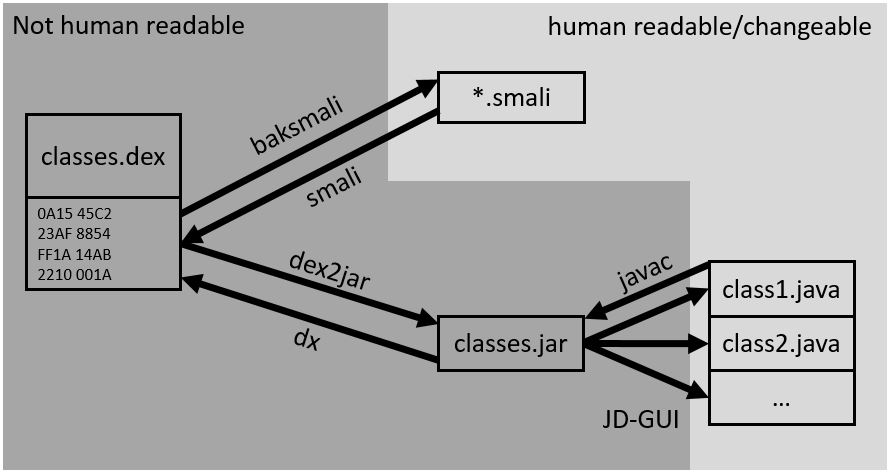
\includegraphics[width=\textwidth]{figures/dex_disassembly}
  \caption[DEX Assembly/Disassembly]{DEX Assembly/Disassembly}
  \label{fig:dex_disassembly}
\end{figure}


\section{Obfuscation Techniques}
Obfuscation in the context of copy protection for application
is generally the term for hardening an application against
reverse code engineering techniques. It can be achieved by different methods
that can be seperated in two main groups, static and dynamic obfuscation.
Static means that the obfuscation technique is applied to code units (source
code, binaries, ...) while the application is not executed. Therefore an
attacker could possibly successful analyze the application without executing it
if he manages to break this obfuscation. Applications that are dynamically
obfuscated on the other hand, are much harder to analyze since the behavior
of the application is not decided until its execution. An attacker needs to connect to the process of the application followed by a just in time inspection.

It does follow a list of common static and dynamic obfuscation techniques
for Android applications.

\subsection{Static}
\subsubsection{Common Source Code Obfuscation}
The most common way of harden source code is to remove any kind of meta data
that has been added during the development process. Means destroying/modifying
information that originally was present in the source code.
This technique can be applied at different layers, \code{.java}, \code{.class} and the final \code{.dex} in case of Android.
Among other things they consist of renaming
classes, variables, functions, irreducable code insertion,
artificial parallelization, method inlining/outlining, unrolling
loops, encoding strings, changing the control flowand so on to confuse code analysts but always keeping its original behavior.

Popular tools for that purpose are Google's ``ProGuard''
\parencite{proguardtool} which is included in the Android build system and
can be enabled easily as well as``DexGuard'' by GuardSquare
\parencite{dexguardtool}. ``ProGuard'' does
operate on source code level where ``DexGuard'' operates on DEX.
Since the first unit of Android applications is Java code, classical Java
obfuscators also can be used.

\subsubsection{Junk-Byte-Insertion}
Junk-Byte-Insertion's goal is to confuse static analyzing
disassembling tools. It does work for tools with the
``linear sweep'' method to analyze a file. That means
the tools are processing every instruction from the entrypoint
till the end without interpreting them (e.g. not following jumps).
That examining technique can be exploited to break the disassembling
procedure. Let's assume we do have the code snippet of
\autoref{fig:junk_byte_listening}
on source code level.

\begin{figure}[htb]
  \centering
  \begin{tabular}{c}
  \begin{lstlisting}[language=Java]
    if (false) {
        0x12 0x34 0x56
    } else {
        proceedProgram()
    }
  \end{lstlisting}
  \end{tabular}
  \caption[Junk-Byte-Insertion]{Junk-Byte-Insertion Example}
  \label{fig:junk_byte_listening}
\end{figure}

Cause of the if-condition, the \code{insertBreakingBytes()} method is never
reached. Since ``linear sweep'' does not perform jumps, the analyzing tool
is trying to revert those bytes into source code. By choosing a specific
sequence of bytes, the transformation will fail.

Enhanced tools will use the ``recursive traversal'' technique to analyze a
file which is capable of detecting dead branches like in the example above.
These tools also may be tricked by choosing a more complicated condition for
if-conditions that can only be evaluated at runtime and therefore the
whole conditional branch (including the breaking byte sequence) would also be evaluated.
\parencite{lvl_imp}.

\subsection{Dynamic}
\subsubsection{Hidden Methods Invocation}
\subsubsection{Dynamic Code Loading}
\subsubsection{Self Modifying Code}

